\let\negmedspace\undefined
\let\negthickspace\undefined
\documentclass[journal]{IEEEtran}
\usepackage[a5paper, margin=10mm, onecolumn]{geometry}
%\usepackage{lmodern} % Ensure lmodern is loaded for pdflatex
\usepackage{tfrupee} % Include tfrupee package

\setlength{\headheight}{1cm} % Set the height of the header box
\setlength{\headsep}{0mm}     % Set the distance between the header box and the top of the text

\usepackage{gvv-book}
\usepackage{gvv}
\usepackage{cite}
\usepackage{amsmath,amssymb,amsfonts,amsthm}
\usepackage{algorithmic}
\usepackage{graphicx}
\usepackage{textcomp}
\usepackage{xcolor}
\usepackage{txfonts}
\usepackage{listings}
\usepackage{enumitem}
\usepackage{mathtools}
\usepackage{gensymb}
\usepackage{comment}
\usepackage[breaklinks=true]{hyperref}
\usepackage{tkz-euclide} 
\usepackage{listings}
% \usepackage{gvv}                                        
\def\inputGnumericTable{}                                 
\usepackage[latin1]{inputenc}                                
\usepackage{color}                                            
\usepackage{array}                                            
\usepackage{longtable}                                       
\usepackage{calc}                                             
\usepackage{multirow}                                         
\usepackage{hhline}                                           
\usepackage{ifthen}                                           
\usepackage{lscape}
\usepackage{circuitikz}
\tikzstyle{block} = [rectangle, draw, fill=blue!20, 
    text width=4em, text centered, rounded corners, minimum height=3em]
\tikzstyle{sum} = [draw, fill=blue!10, circle, minimum size=1cm, node distance=1.5cm]
\tikzstyle{input} = [coordinate]
\tikzstyle{output} = [coordinate]
\begin{document}
\textbf If a line has the direction ratios $-18,\, 12,\, -4$, then what are its direction cosines?

\vspace{1em}

\textbf{Solution:} Let
\[
\mathbf{A} = \begin{pmatrix}
-18 \\
12 \\
-4
\end{pmatrix}.
\]

The direction cosines of the line are the components of the unit vector in the direction of $\mathbf{A}$. To find this, we first calculate the norm of $\mathbf{A}$:
\[
\|\mathbf{A}\| = \sqrt{(-18)^2 + 12^2 + (-4)^2} = \sqrt{324 + 144 + 16} = \sqrt{484} = 22.
\]

Next, dividing each component of $\mathbf{A}$ by $\|\mathbf{A}\|$ gives the unit direction vector:
\[
\frac{\mathbf{A}}{\|\mathbf{A}\|} = \frac{1}{22} \begin{pmatrix}
-18 \\
12 \\
-4
\end{pmatrix} = \begin{pmatrix}
-\frac{9}{11} \\
\frac{6}{11} \\
-\frac{2}{11}
\end{pmatrix}.
\]




\begin{figure}[H]
    \centering
    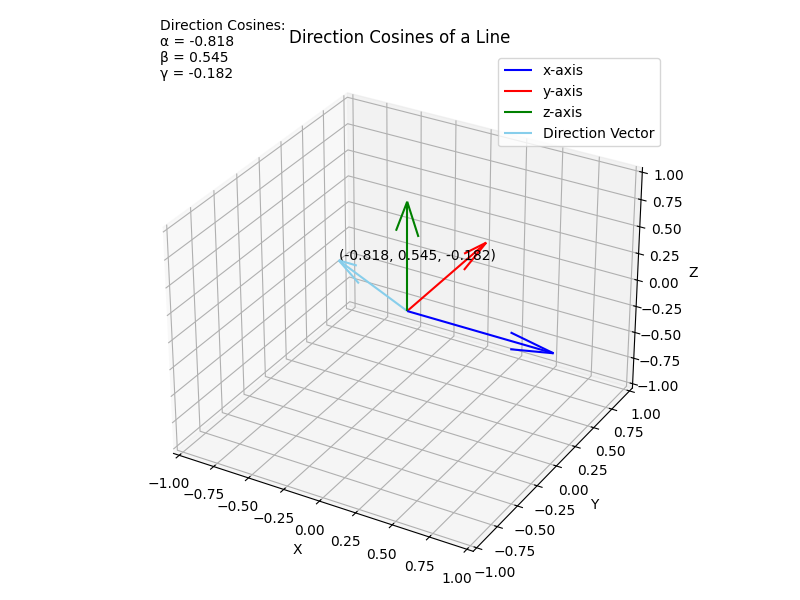
\includegraphics[width=1\linewidth]{figs/plot.png}
    \caption{plot}
    \label{fig:placeholder}
\end{figure}
\end{document}
